\Exhibit{ThomsenFollowers}{%
    Сравнение подписчиков на Medium у Алексея Инкина и Michael Thomsen, менеджера продуктов,
    официально объявляющего о новых релизах%
}

У Алексея Инкина больше 600 подписчиков:
\begin{center}
    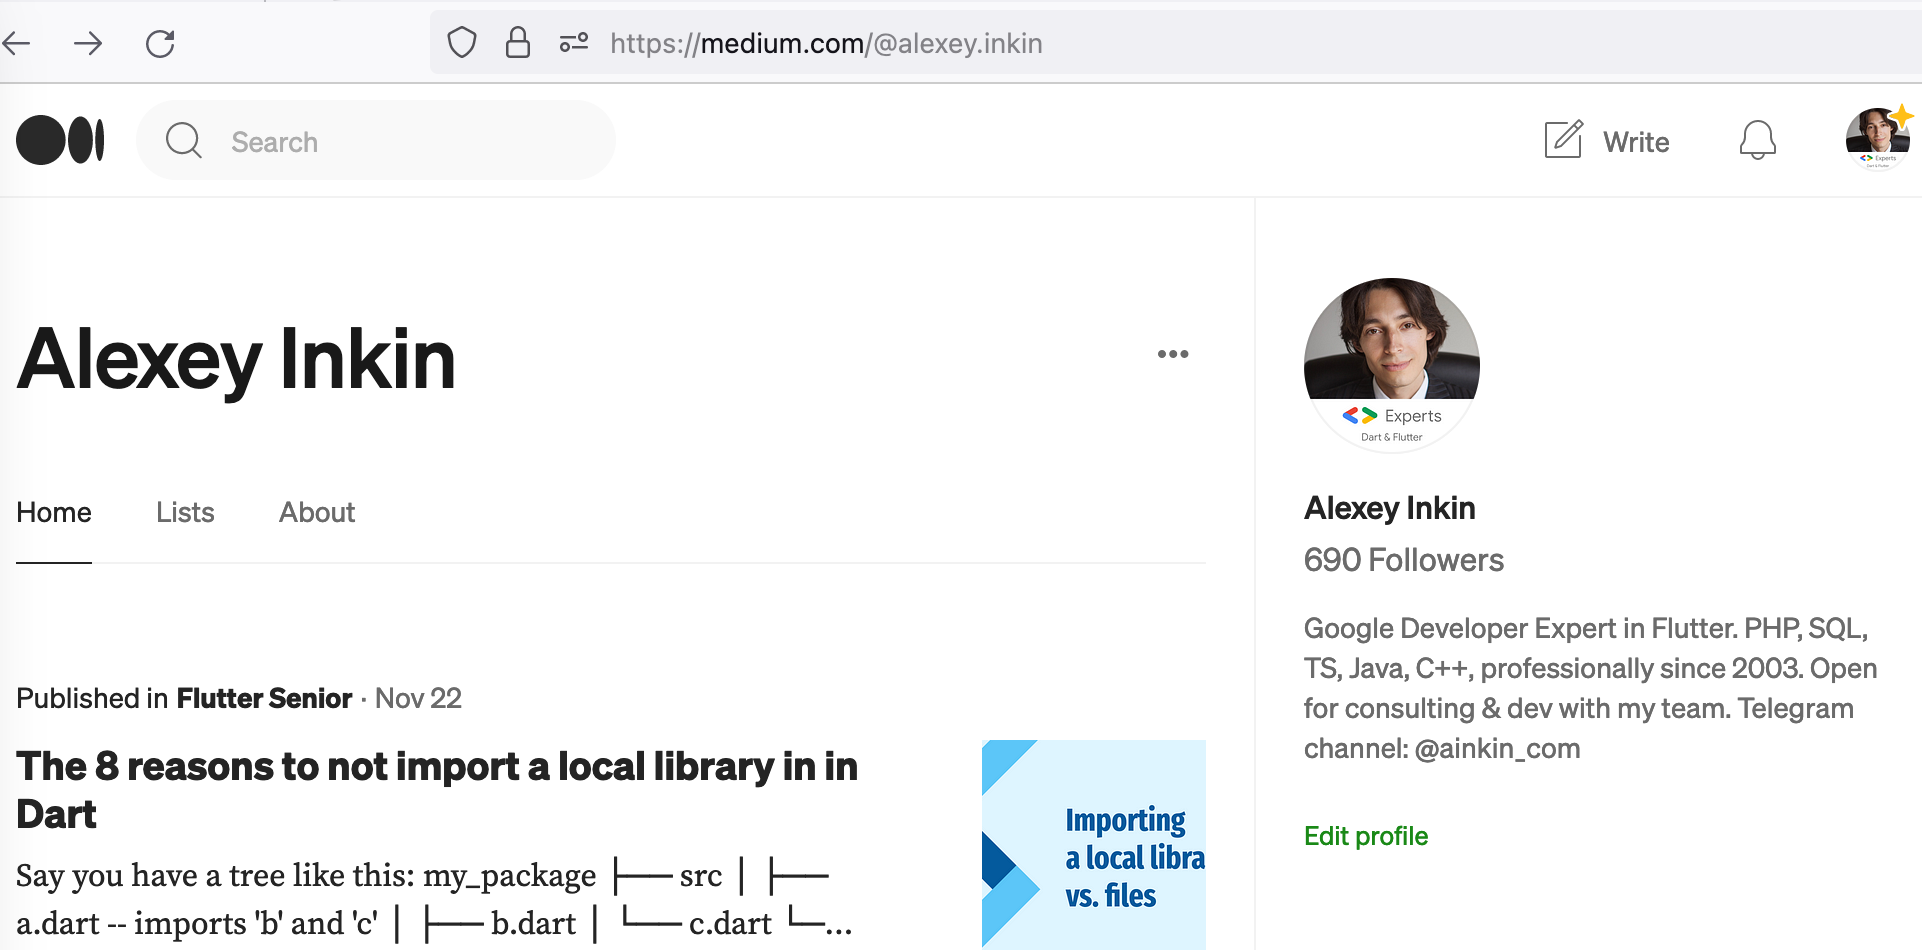
\includegraphics[width=35em]{inkin-followers}
\end{center}

Для сравнения у Michael Thomsen чуть больше 6 тысяч подписчиков (см. скриншот ниже).
Из его профиля видно, что он менеджер продуктов Dart и Flutter,
и он публикует официальные анонсы о новых релизах Dart.

\begin{center}
    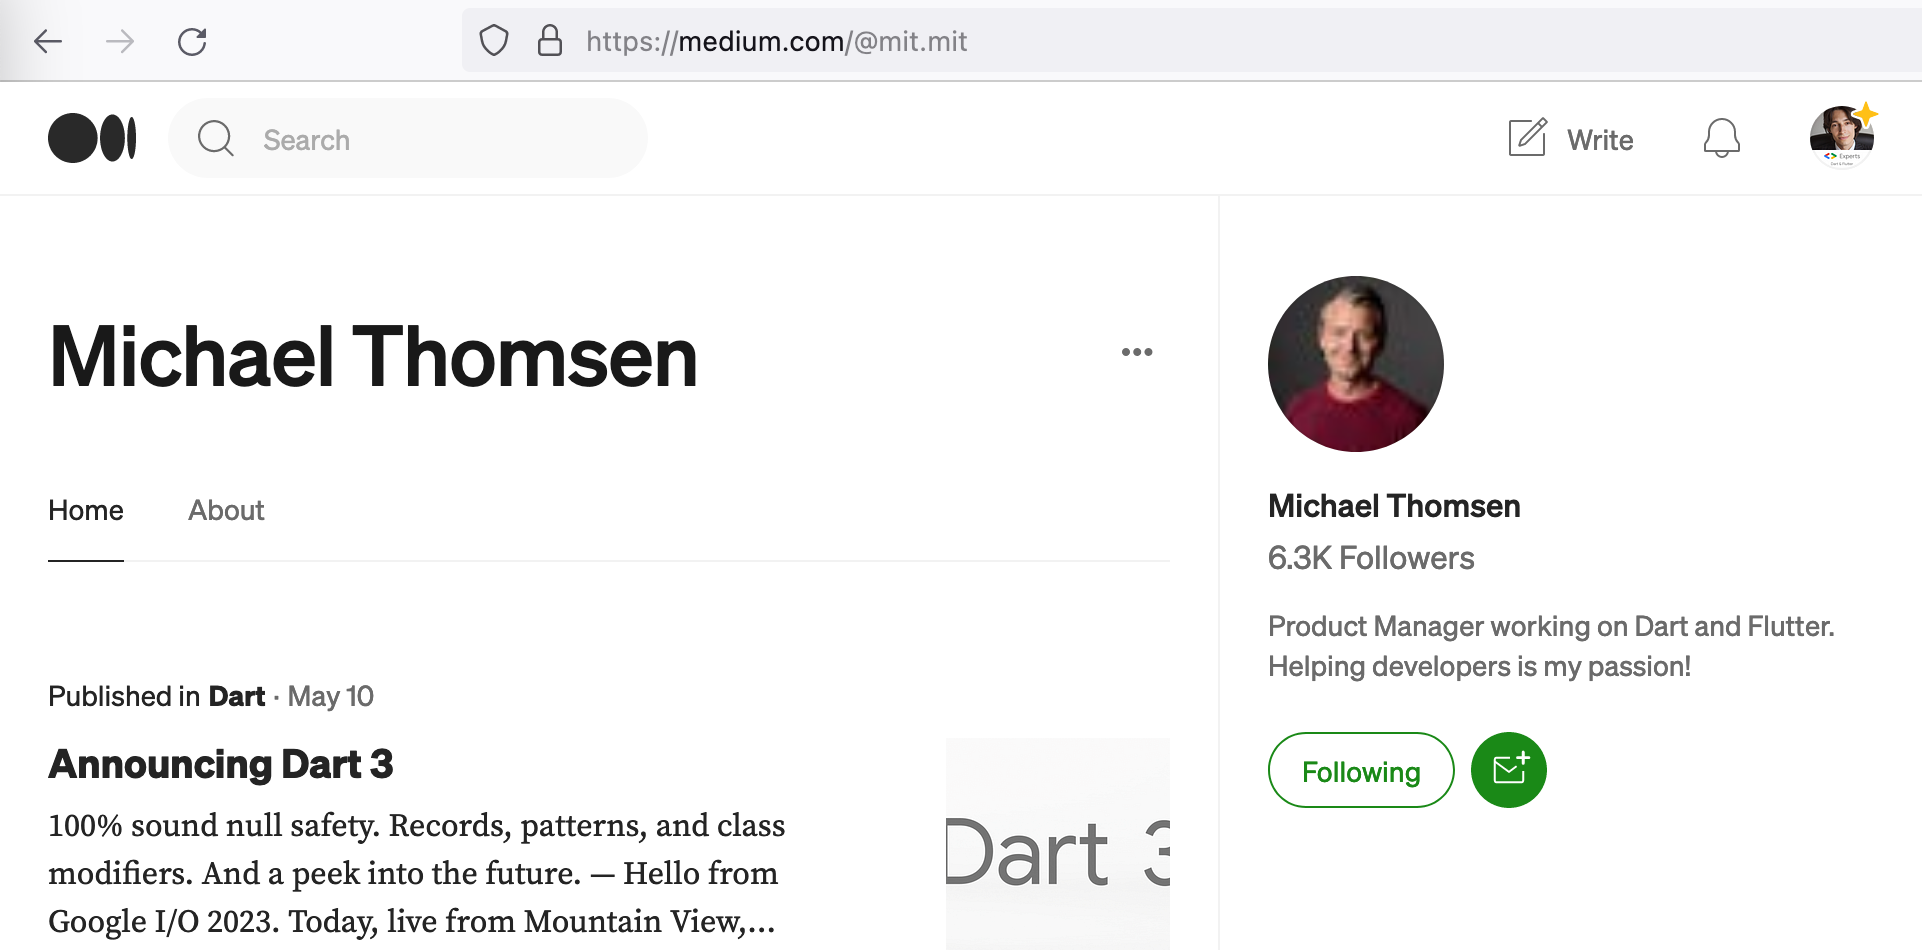
\includegraphics[width=35em]{thomsen-followers-p1}
\end{center}
\WillContinue
\pagebreak

\Continuing
\begin{center}
    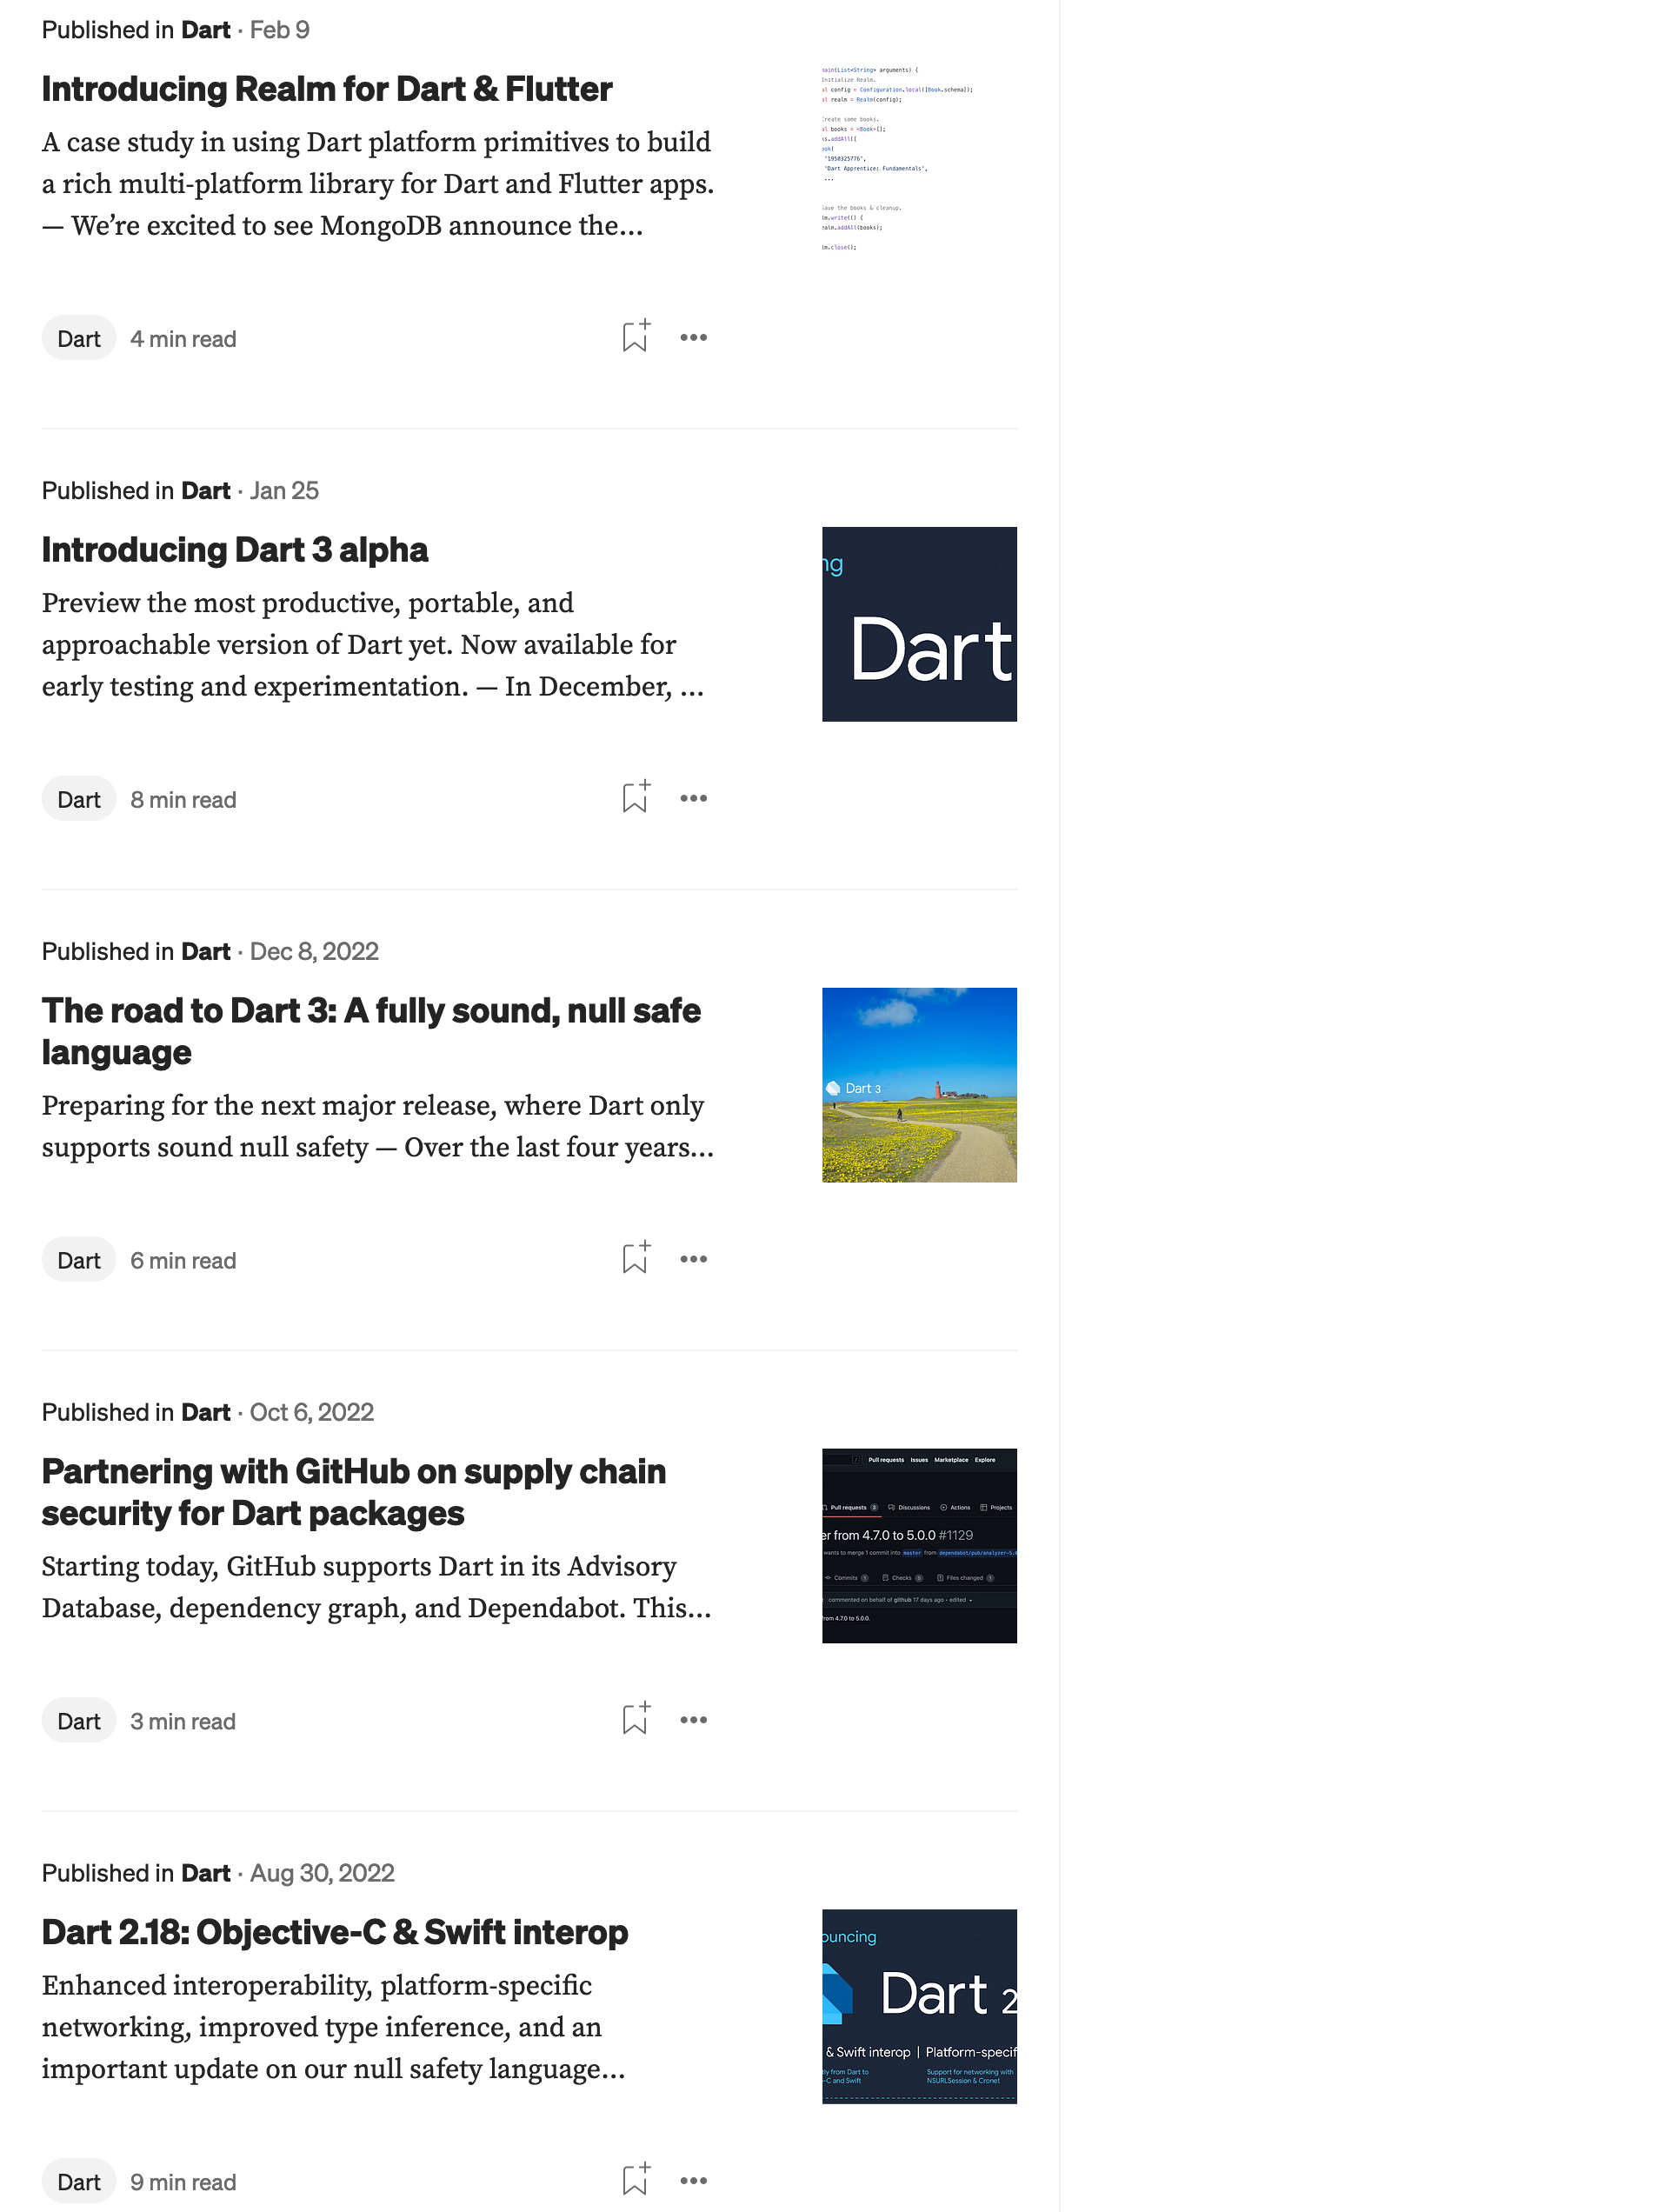
\includegraphics[width=35em]{thomsen-followers-p2}
\end{center}

Если у технического писателя всего в 10 раз меньше подписчиков, чем у менеджера языка,
о котором он пишет, то его статьи должны считаться успешными после всего двух лет публикаций.

\pagebreak
